\renewcommand{\theequation}{\theenumi}
\begin{enumerate}[label=\arabic*.,ref=\thesubsection.\theenumi]
\numberwithin{equation}{enumi}

\item Find the circumcentre $\vec{O}$ and radius $R$ of $\triangle ABC$ in Fig. \ref{fig:triangle}
\\
\solution $\vec{O}$ can be obtained from 
%
The following code computes $\vec{O}$ using \eqref{eq:defs_ccircle_c1} and \eqref{eq:defs_ccircle_c2}
\begin{lstlisting}
https://raw.githubusercontent.com/gadepall/school/master/linalg/book/codes/circumcentre.py
\end{lstlisting}
\item Plot the circumcircle of $\triangle ABC$.
\\
\solution The following code plots Fig. \ref{fig:circumcircle}
\begin{lstlisting}
https://raw.githubusercontent.com/gadepall/school/master/linalg/book/codes/circumcircle.py
\end{lstlisting}
\begin{figure}
\centering
\includegraphics[width=\columnwidth]{./circle/figs/circumcircle.eps}
\caption{}
\label{fig:circumcircle}
\end{figure}


\item Consider a circle with centre $\vec{I}$ and radius $r$ that lies within $\triangle ABC$ and touches 
$BC, CA$ and $AB$ at $\vec{U}, \vec{V}$ and $\vec{W}$ respectively.

\item Compute $\vec{I}$ and $r$.
\\
\solution The following code uses \eqref{eq:incirc_k1k2fin}  and \eqref{eq:incirc_rad} to compute $\vec{I}$ and  $r$ respectively.


\begin{lstlisting}
https://raw.githubusercontent.com/gadepall/school/master/linalg/book/codes/incentre.py
\end{lstlisting}
\item Plot the incircle of $\triangle ABC$
\\
\solution The following code plots the incircle in Fig. \ref{fig:incircle}
\begin{lstlisting}
https://raw.githubusercontent.com/gadepall/school/master/linalg/book/codes/incircle.py
\end{lstlisting}
\begin{figure}
\centering
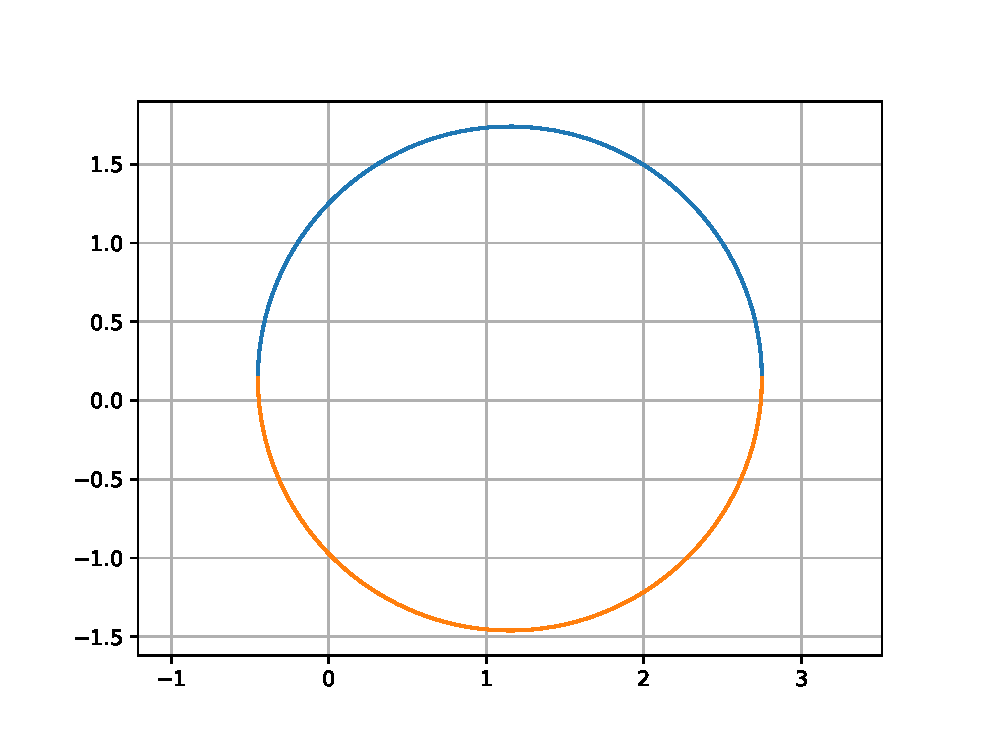
\includegraphics[width=\columnwidth]{./circle/figs/incircle.eps}
\caption{}
\label{fig:incircle}
\end{figure}

\end{enumerate}


